\documentclass[12pt]{article}
\usepackage[pdfborder={0 0 0.5 [3 2]}]{hyperref}%
\usepackage[left=1in,right=1in,top=1in,bottom=1in]{geometry}%
\usepackage[shortalphabetic]{amsrefs}%
\usepackage{amsmath}
\usepackage{enumerate}
\usepackage{enumitem}
\usepackage{amssymb}                
\usepackage{amsmath}                
\usepackage{amsfonts}
\usepackage{amsthm}
\usepackage{bbm}
\usepackage[table,xcdraw]{xcolor}
\usepackage{tikz}
\usepackage{float}
\usepackage{booktabs}
\usepackage{svg}
\usepackage{mathtools}
\usepackage{cool}
\usepackage{url}
\usepackage{graphicx,epsfig}
\usepackage{framed}
\usepackage{hyperref}  

\usetikzlibrary{automata,arrows,positioning,calc}
\DeclarePairedDelimiter\abs{\lvert}{\rvert}%
\DeclarePairedDelimiter\norm{\lVert}{\rVert}%
\DeclarePairedDelimiter\ceil{\lceil}{\rceil}
\DeclarePairedDelimiter\floor{\lfloor}{\rfloor}

\makeatletter
\renewcommand*\env@matrix[1][*\c@MaxMatrixCols c]{%
  \hskip -\arraycolsep
  \let\@ifnextchar\new@ifnextchar
  \array{#1}}
\makeatother

\newtheorem{theorem}{Theorem}[section]
\newtheorem{corollary}{Corollary}[theorem]
\newtheorem{proposition}[theorem]{Proposition}
\newtheorem{lemma}[theorem]{Lemma}

\theoremstyle{definition}
\newtheorem{definition}[theorem]{Definition}
\newtheorem{exercise}{Exercise}%
\newtheorem{problem}[exercise]{Problem}%
\newtheorem*{example}{Example}

\theoremstyle{remark}
\newtheorem*{question}{Question}
\newtheorem*{observation}{Observation}
\newtheorem*{remark}{Remark}

\graphicspath{ {images/} }

\setlength{\parindent}{0cm}
\renewcommand{\vec}[1]{\ensuremath{\mathbf{#1}}}

\def\noi{\noindent}
\def\T{{\mathbb T}}
\def\R{{\mathbb R}}
\def\N{{\mathbb N}}
\def\C{{\mathbb C}}
\def\Z{{\mathbb Z}}
\def\P{{\mathbb P}}
\def\E{{\mathbb E}}
\def\Q{\mathbb{Q}}
\def\ind{{\mathbb I}}

\def\cale{{\mathcal E}}
\def\cals{{\mathcal S}}
\def\calc{{\mathcal C}}
\def\caln{{\mathcal N}}
\def\calb{{\mathcal B}}
\def\calg{{\cal G}}

\def\ds{\displaystyle}
\def\ra{\rightarrow}
\newcommand{\conv}{\mbox{\rm conv}}
\newcommand{\spaan}{\mbox{\rm span}}
\newcommand{\deet}{\mbox{\rm det}}
\newcommand{\aff}{\mbox{\rm aff}}
\newcommand{\cl}{\mbox{\rm cl}}
\newcommand{\dimm}{\mbox{\rm dim}}
\newcommand{\sm}{\setminus}
\def\ci{\perp\!\!\!\perp}

\newcommand{\ink}{\rule{.5\baselineskip}{.55\baselineskip}}

\begin{document}

\setcounter{section}{1}
\section{Discrete Random Variables}

\subsection{Random Variables}
A \emph{random variable} is a real-valued function on a sample space\footnote{It's not really a variable at all, but we are stuck with the terminology.|}. The random variable generally is a quantity we wish to measure; the output of the random variable depends on which element of the sample space is chosen. Random variables are designated by uppercase letters, e.g. $X$ and $Y$.\\

In this section, we will look at discrete random variables.

\begin{framed}
A \emph{discrete} random variable $Y$ is a random variable which can only take on a finite or countable set of distinct values.
\end{framed}

Here are some examples of discrete random variables:
\begin{enumerate}
\item The number of voters in Rhode Island who prefer Hillary Clinton.
\item The number of defective lightbulbs out of a shipment of 1000 lightbulbs.
\item The number of times I play a slot machine in Las Vegas until I win.
\end{enumerate}

We will use the following simple example to illustrate features of discrete random variables.

\begin{example}Let $\cals$ be the sample space representing the flip of two fair coins. Let $Y$ be the number of heads flipped. Then $Y$ is a discrete random variable, since it can only have the values 0, 1, or 2. We can illustrate it graphically below.
\begin{figure}[H]
\centering
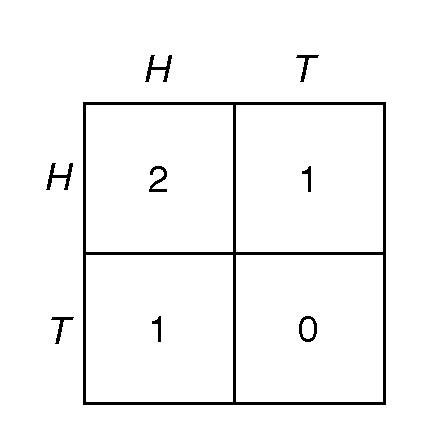
\includegraphics[width=3cm]{numberofheads.eps}
\end{figure}
\end{example}

Uppercase letters, such as $Y$, are used to designate random variables. We use lowercase letters, such as $y$, to designate a value that a random variable can take. The expression $(Y = y)$ is shorthand for the set of all points in our sample space $\cals$ for which the random variable $Y$ outputs the value $y$. Since $(Y = y)$ is a subset of $\cals$, it is an event in our sample space. In the two-coin-toss problem, for example, the possible values of $Y$ are 0, 1, and 2, so we have:
\begin{itemize}[noitemsep]
\item $(Y = 0) = \{ (T, T) \}$
\item $(Y = 1) = \{ (H, T), (T, H) \}$
\item $(Y = 2) = \{ (H, H) \}$
\end{itemize}

Since $(Y = y)$ is an event in our sample space, we can talk about its probabiltiy, i.e. $\P(Y = y)$. In fact, the point of random variables is to do just this! 

\begin{framed}
  \emph{Probability of a discrete random variable }\\
  \rule{\dimexpr\linewidth-2\fboxsep-2\fboxrule}{.1pt} \\
  The probability that a discrete random variable $Y$ takes the value $y$, denoted $\P(Y = y)$, or $p(y)$ for short, is the probability of the event $(Y = y)$, the set of all points in the sample space $\cals$ which output the value $y$. \\

  $\P(Y = y)$ is the sum of the probabilities of all the simple events in $\cals$ which are assigned the value $y$ by the random variable $Y$.
\end{framed}

Back to our two-coin-toss problem, let's look at the probabilties of the random variable $Y$. For convenience, here is a picture of the sample space probabilities next to a graphical representation of $Y$. Since we are using the discrete uniform distribution for coin tosses, each simple event in our sample space has probability 1/2.
\begin{figure}[H]
\centering
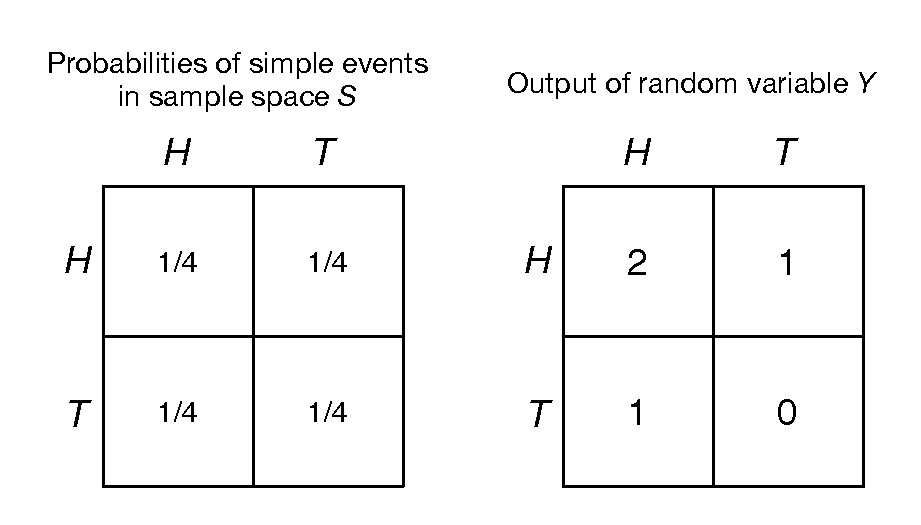
\includegraphics[width=8cm]{numberofheads2.eps}
\end{figure}

Using the rule above, we can compute the following probabilties for $Y$ by adding up the probabilities of the underlying simple events. In this case, since we are using the discrete uniform distribution, we could also just count the number of simple events which lead to each output of $Y$ and divide by 4, the size of the sample space.
\begin{itemize}[noitemsep]
\item $\P(Y = 0) = 1/4$
\item $\P(Y = 1) = 1/4 + 1/4 = 1/2$
\item $\P(Y = 2) = 1/4$
\end{itemize}


\begin{framed}
  \emph{Probability mass function }\\
  \rule{\dimexpr\linewidth-2\fboxsep-2\fboxrule}{.1pt} \\
  The \emph{probablity mass function (pmf)} is a function which gives the probabiltiy that a discrete random variable $Y$ is exactly equal to a value $y$. The pmf can be represented as a function, table, or graph which gives the values $p(y) = \P(Y = y)$ for all possible values $y$ which $Y$ can take.
\end{framed}

In the two-coin-flip example, we can represent the pmf of $Y$ in a table:
\begin{figure}[H]
\centering
\begin{tabular}{l@{\hskip 2cm}l}
\toprule
$y$ & $p(y)$\\
\midrule
0 & 1/4\\
1 & 1/2\\
2 & 1/4\\
\bottomrule
\end{tabular}
\end{figure}

A discrete random variable induces a probability distribution on the sample space of all possible values the random variable can take. This is a different sample space from the original sample space. Back to our two-coin-flip example, the random variable $Y$ induces a probability distribution on a new sample space $\mathcal{T} = \{0, 1, 2\}$. The probabilities of the sample points in $\mathcal{T}$ are the probabilties $p(y)$ for $y = 0, 1, 2$. We can illustrate this new sample space in a picture.

\begin{figure}[H]
\centering
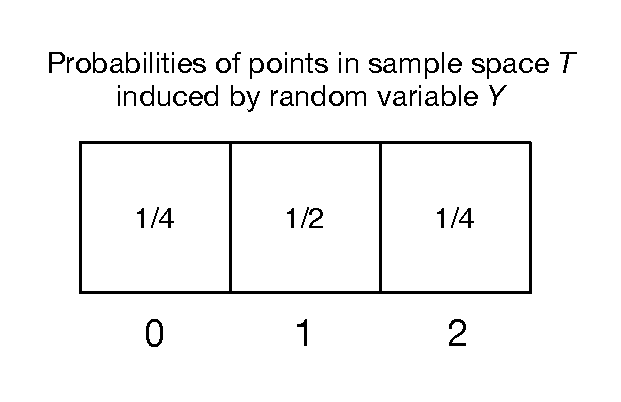
\includegraphics[width=5cm]{induced1.eps}
\end{figure}

Often (as we shall see), we care much more about the sample space induced by a random variable than the underlying sample space. Since a discrete random variable induces a probability distribution, the following must be true.

\begin{framed}
For any discrete random variable $Y$:
\begin{align*}
0 \leq p(y) &\leq 1 \:\text{ for all }y \\
\sum_{\text{all } y} p(y) &= 1
\end{align*}
where $p(y) = \P(Y = y)$. Since we have a discrete sample space, the sum is finite or countable.
\end{framed}

Let's look at two more examples, this time involving the rolls of two six-sided dice.

\begin{example}Let $\cals$ be the sample space representing the rolls of two six-sided dice. Consider the following two random variables:
\begin{enumerate}
\item $X$ = the sum of the two dice
\item $Y$ = the larger of the two die rolls (if they are the same, then it's just equal to both die rolls)
\end{enumerate} 
Let's look at these random variables graphically.
\begin{figure}[H]
\centering
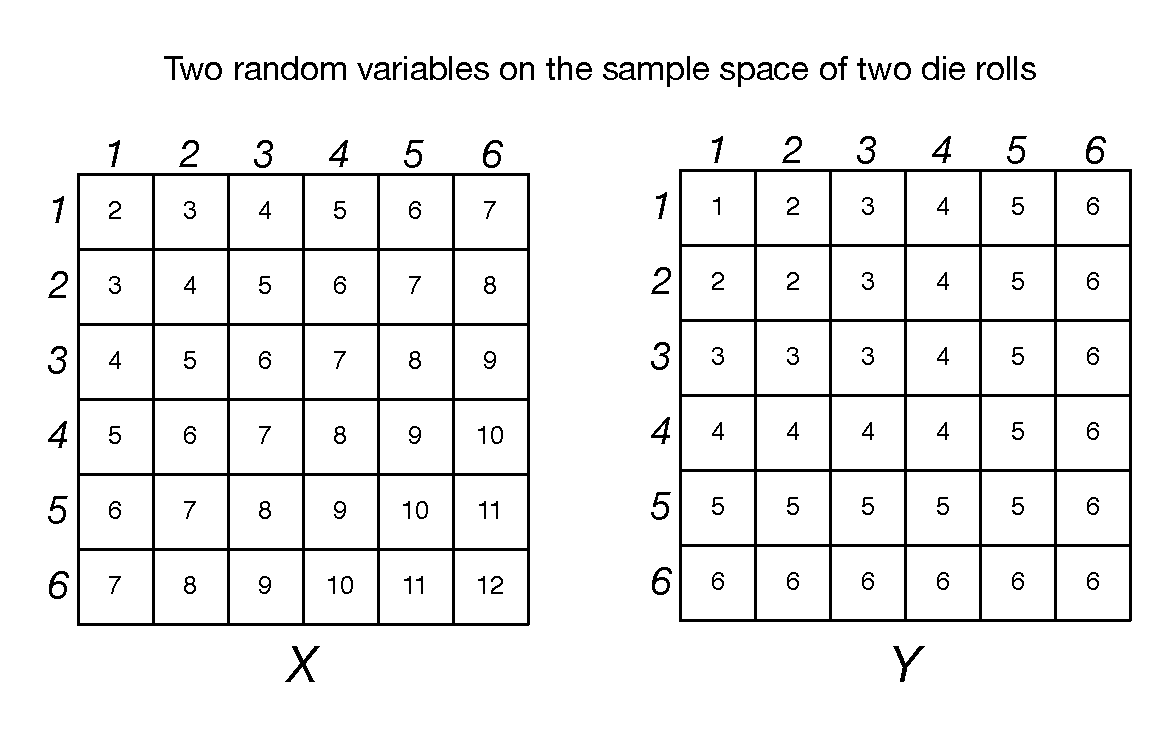
\includegraphics[width=8cm]{2dicervs.eps}
\end{figure}
\end{example}

\end{document}